\section{Lektion 08-02-2018}

\begin{enumerate}
	\item Mikrofon
	\item Højtaler (afstandsregel)
	\item Måling af lydtryk
\end{enumerate}

\begin{mdframed}[style=exampledefault]
	\begin{itemize}
		\item \textbf{Pensum:} 
		\begin{enumerate}
			\item Audio Meetering, sec. 8-9, 26-29
			\item Elektroakustik, TAS,  p. 12-14
		\end{enumerate}
		\item \textbf{Opgaver:} 
		\begin{enumerate}
			\item Lyd og Akustik - Lektion 2 - opgaver og øvelser
		\end{enumerate}
	\end{itemize}
\end{mdframed}

\subsection{Mikrofon}
\begin{itemize}
	\item En transducer der omsætter et oscillerende lydtryk til et analogt elektrisk signal.
	\begin{itemize}
		\item Kaldes også for en tryktransducer.
		\item Måler lydtrykkets variation i et punkt uden reference til den retning lyden udbredes i.
		\item Flere mikrofontyper er retningsbestemte på grund af deres opbygning.
	\end{itemize}
\end{itemize}

\subsubsection{Kondensator mikrofon}
\begin{itemize}
	\item En tynd membran af udspændt metalfolie er anbragt tæt på
	en fastsiddende elektrode.
	\item Kondensatoren mellem membran og elektrode oplades gennem $R_p$. 
	\item Spændingen mellem membran og elektrode vil variere efter definitionsligningen $Q = C\cdot U$.
	\begin{itemize}
		\item $Q$ er den konstante ladning givet af polarisationsspændingen $U_P$ der ved målemikrofoner typisk er \SI{200}{\volt}.
	\end{itemize}
	\item Den lave grænsefrekvens sættes af $R_p$ og mikrofonens kapacitet $C$.
	\begin{itemize}
		\item $C \approx \SI{5}{\pico\farad}-\SI{20}{\pico\farad}$ gør at  $R_p$ skal være mindst \SI{1}{\giga\ohm} for måling af hørbar lyd.
	\end{itemize}
	\item Den høje grænsefrekvens sættes af membranens masse. 
\end{itemize}

\begin{figure} [H]
	\centering
	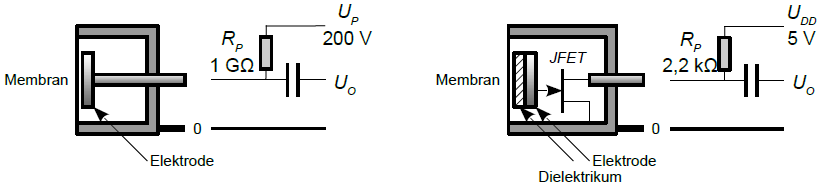
\includegraphics[width=\linewidth]{graphics/11.png}
	\caption{Kondensatormikrofons opbygning.}
	\label{fig:11}
\end{figure}

\begin{itemize}
	\item Alternativt indbygges en plastskive mellem membran og elektrode hvor en såkaldt "fastfrosset ladning" fungerer som $Q$.
	\item Den høje udgangsimpedans sænkes af en indbygget JFET og det eksterne kredsløb skal nu levere strøm til transistorens drain.
	\item Følsomheden er typisk $\approx 5 \si{\milli\volt}/\si{\pascal}$. 
\end{itemize}

\subsubsection{Dynamisk mikrofon}
\begin{itemize}
	\item \textbf{Klassiske form}: minder om en højttaler (membranen sættes i bevægelse af lydtrykket). Derved bevæges svingspolen i magnetfeltet
	og der induceres en spænding.
	\item \textbf{Båndmikrofonen}: membranen er i et kraftigt magnetfelt. Når lydtrykket får membranen til at svinge induceres der en spænding over de to ender af båndet. Spændingen er normalt så lav at der skal benyttes en transformator for at løfte det op på et brugbart niveau. 
	\begin{itemize}
		\item Lyden har adgang til begge sider af membranen.
		\begin{itemize}
			\item Mest følsom for lyd på aksen ($0\degree$ og $180\degree$.
			\item Der kan ikke registreres lyd fra siden ($90\degree$).
		\end{itemize}
	\end{itemize} 
\end{itemize}
\begin{figure} [H]
	\centering
	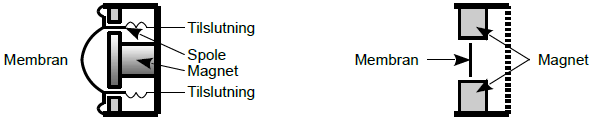
\includegraphics[width=.9\linewidth]{graphics/12.png}
	\caption{(V: svingspolen drives af en membran til at svinge i et magnetfelt.) (H: En tynd metalfolie svinger i et magnetfelt og signalet tages ud ved båndets ender (ud af papiret og ind i papiret)).}
	\label{fig:12}
\end{figure}

\subsection{Højtaler (afstandsregel)}
\fxnote{Mangler højtaler (aftandsregel) noter.}

\subsection{Måling af lydtryk}
\fxnote{Mangler måling af lydtryk noter.}

\subsection{Opgaver}

\begin{enumerate}
	\item Lav et MLS signal med orden 10.
	\item Find impulsresponsen ud fra de sammenhørende exitations- og målesignaler i filen meassigs.mat. Systemet er ”målt” både med MLS og hvid støj.
	\item En 8 ohms højttaler har DC modstand på 6 ohm og virkningsgrad på 1 \%.
	\begin{enumerate}
		\item Bestem den producerede akustiske effekt, når højttaleren tilføres 2,83 volt.
		\item Lyden antages at udbrede sig sfærisk fra højttaleren. Beregn intensiteten og lydtrykniveauet på 2,5 meters afstand.
		\item Lydtrykket måles nu med en mikrofon hvis følsomhed er 5 mV/Pa. Hvilken spænding leverer mikrofonen?
	\end{enumerate}
\end{enumerate}


\begin{lstlisting}
%% LYAK L2 08-02-2018

\end{lstlisting}

